\section{Methodology}
\label{sec:methodology}

Figure \ref{fig:methodology} depicts the phases of the scientific research process that will guide the development of this thesis: Problem Statement, Hypothesis Construction, Experimentation, Conclusion, and Publication. Problem Statement, for identifying and establishing the research question. Hypothesis Construction, for formulating the hypothesis and the associated fundamental questions. In addition, this phase aims to define and carry out the conceptual and technological approaches. Experimentation, for testing the hypothesis and analyzing the evaluation results. Conclusion, for outlining conclusions and future works. Note that Hypothesis Construction has feedback from Experimentation and Conclusion. Publication, for submitting and publishing papers for renowned conferences and journals. The writing of the dissertation document also belongs to this last phase.

\begin{figure}[!ht]
    \centering
    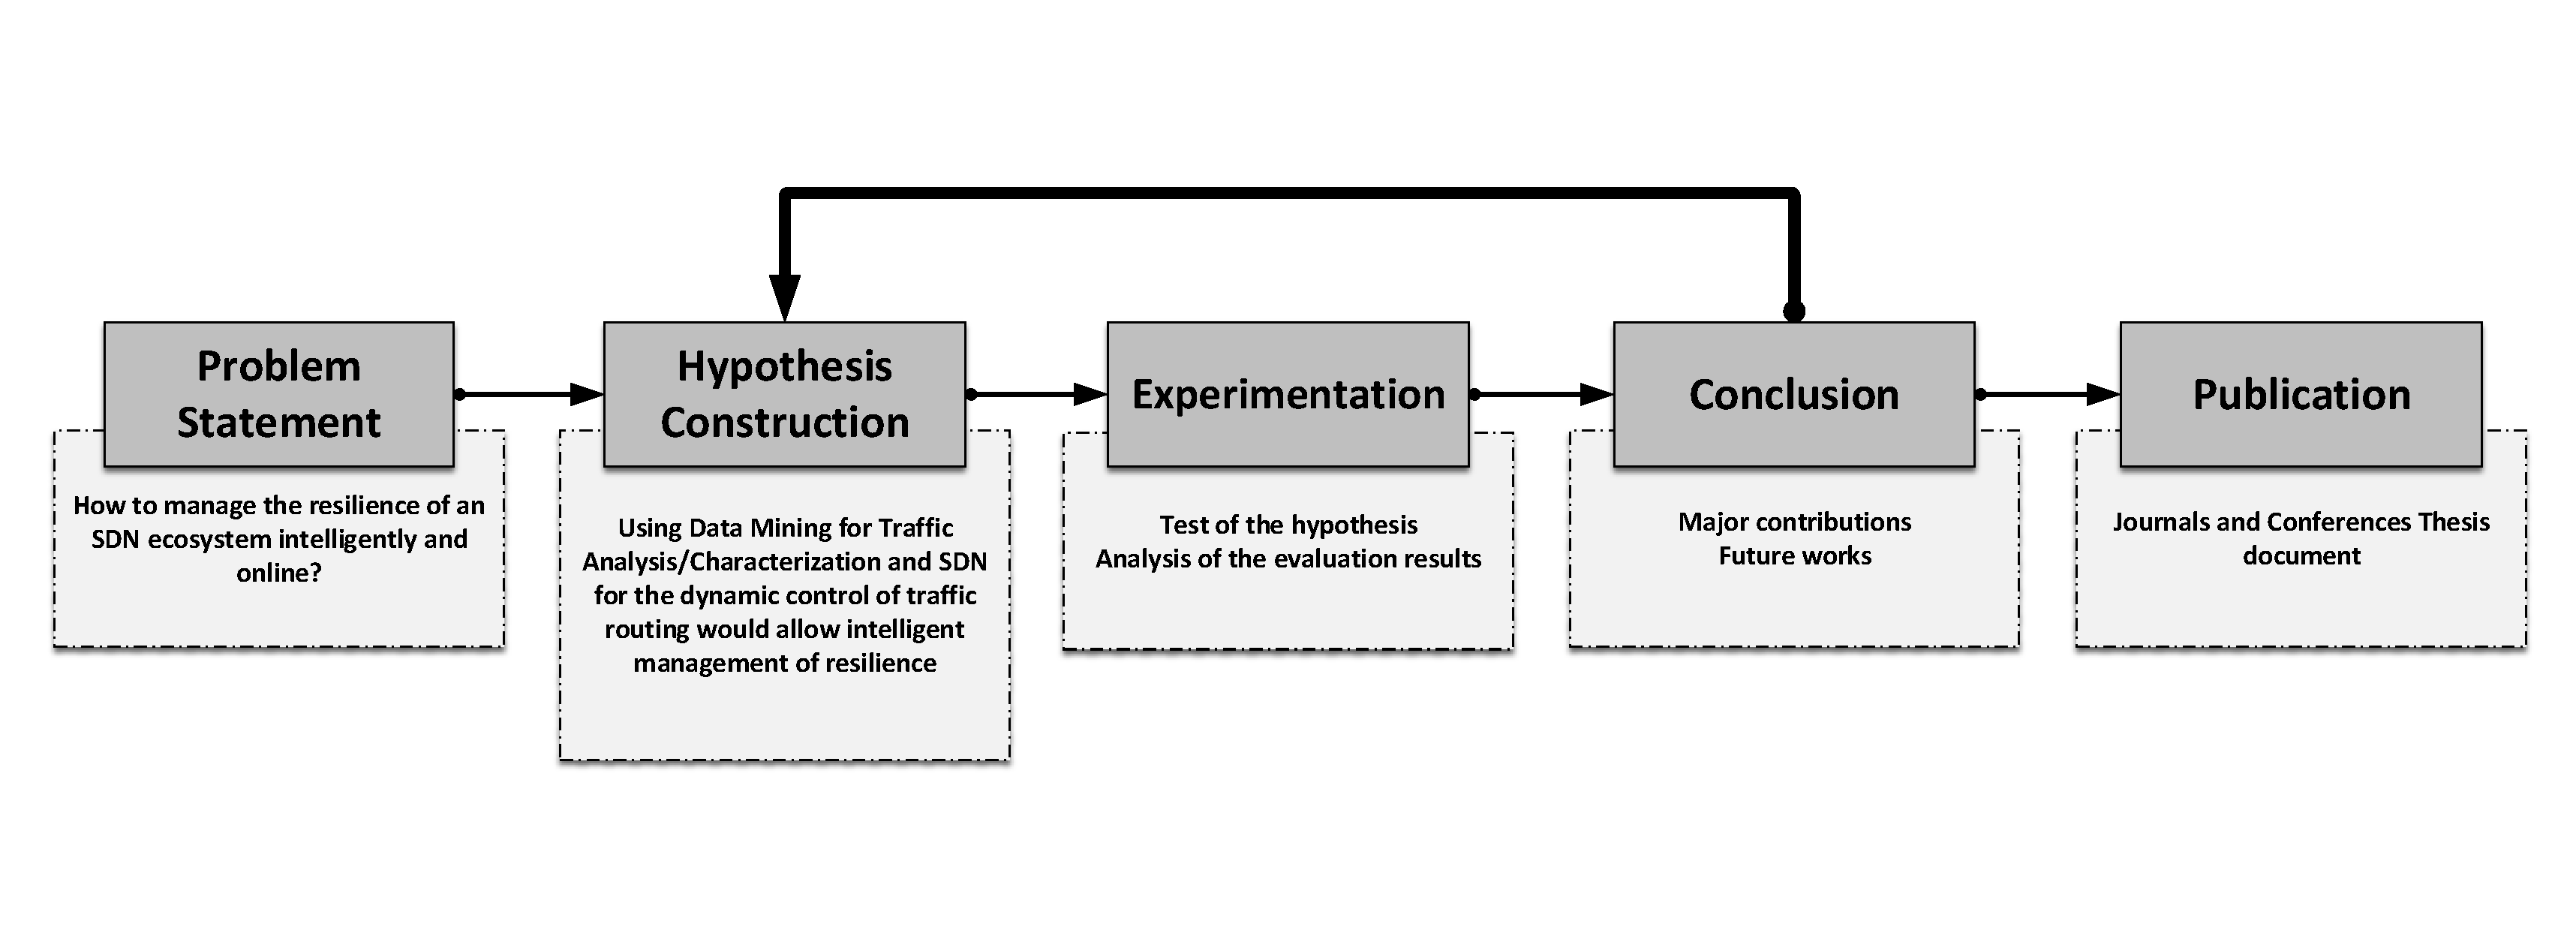
\includegraphics[width=1\columnwidth]{scientific_research_process}
    \caption{Thesis phases}
    \label{fig:scientific_research_process}
\end{figure}